\chapter{Sequences of Functions} \label{fs:chapter}

%%%%%%%%%%%%%%%%%%%%%%%%%%%%%%%%%%%%%%%%%%%%%%%%%%%%%%%%%%%%%%%%%%%%%%%%%%%%%%

\section{Pointwise and uniform convergence}
\label{sec:puconv}

\sectionnotes{1--1.5 lecture}

Up till now, when we talked about limits of sequences we talked about
sequences of numbers.
A very useful concept in analysis is a sequence of functions.
For example, a solution to some differential equation
might be found by finding only approximate solutions.
Then the actual solution is some sort of limit of those approximate solutions.

When talking about sequences of functions, the 
tricky part is that there are multiple notions of a limit.
Let us describe two common
notions of a limit of a sequence of functions.

\subsection{Pointwise convergence}

\begin{defn}
\index{pointwise convergence}
For every $n \in \N$,
let $f_n \colon S \to \R$ be a function.  The sequence
$\{ f_n \}_{n=1}^\infty$
\emph{\myindex{converges pointwise}}\footnote{Unless otherwise specified,
\emph{converges} generally means \emph{converges pointwise}.}
to $f \colon S \to \R$ if for every $x
\in S$,
we have
\begin{equation*}
f(x) =
\lim_{n\to\infty} f_n(x) .
\end{equation*}
\end{defn}

Limits of sequences of numbers are unique, and so if a sequence
$\{ f_n \}_{n=1}^\infty$
converges pointwise, the limit function $f$ is unique.
It is common to say that $f_n \colon S \to \R$
\emph{converges pointwise to $f$ on $T \subset S$}
for some $f \colon T \to \R$.  In that case we mean 
$f(x) = \lim_{n\to\infty} f_n(x)$ for every $x \in T$.  In other words, the
restrictions of $f_n$ to $T$ converge pointwise to $f$.


\begin{example}
On $[-1,1]$, the sequence of functions defined by $f_n(x) \coloneqq x^{2n}$
converges pointwise to $f \colon [-1,1] \to \R$, where
\begin{equation*}
f(x) =
\begin{cases}
1 & \text{if } x=-1 \text{ or } x=1, \\
0 & \text{otherwise.}
\end{cases}
\avoidbreak
\end{equation*}
See \figureref{x2nfig}.

\begin{myfigureht}
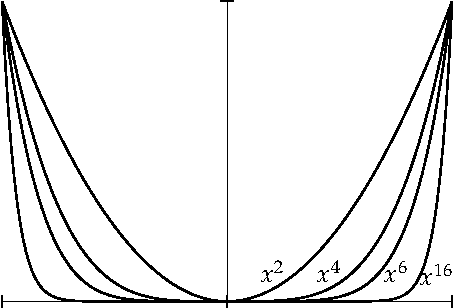
\includegraphics{figures/x2nfig}
\caption{Graphs of $f_1$, $f_2$, $f_3$, and $f_8$ for $f_n(x) \coloneqq
x^{2n}$.\label{x2nfig}}
\end{myfigureht}

To see this is so, first take $x \in (-1,1)$.  Then 
$0 \leq x^2 < 1$.
We have seen before that
\begin{equation*}
\abs{x^{2n} - 0} = {(x^2)}^n \to 0 \quad \text{as} \quad n \to \infty .
\end{equation*}
Therefore, $\lim_{n\to\infty}f_n(x) = 0$.

When $x = 1$ or $x=-1$, then $x^{2n} = 1$ for all $n$ and hence
$\lim_{n\to\infty}f_n(x) = 1$.
For all other $x$, the sequence
$\bigl\{ f_n(x) \bigr\}_{n=1}^\infty$ does not converge.
\end{example}

Often, functions are given as a series.  In this case, we use
the notion of pointwise convergence to find the values of the function.

\begin{example} \label{example:geomsumptconv}
We write
\begin{equation*}
\sum_{k=0}^\infty x^k
\end{equation*}
to denote the limit of the functions
\begin{equation*}
f_n(x) \coloneqq \sum_{k=0}^n x^k .
\end{equation*}
When studying series, 
we saw that for $(-1,1)$ the $f_n$ converge pointwise to
\begin{equation*}
\frac{1}{1-x} .
\end{equation*}

The subtle point here is that while
$\frac{1}{1-x}$ is defined for all $x \not=1$, and $f_n$ are 
defined for all $x$ (even at $x=1$), convergence only happens on $(-1,1)$.
Therefore, when we write
\begin{equation*}
f(x) \coloneqq \sum_{k=0}^\infty x^k
\end{equation*}
we mean that $f$ is defined on $(-1,1)$ and is the pointwise limit
of the partial sums.
\end{example}

\begin{example}
Let $f_n(x) \coloneqq \sin(nx)$.  Then $f_n$ does not converge pointwise
to any function on any interval.  It may converge at certain points, such
as when $x=0$ or $x=\pi$.  It is left as an exercise that in any interval
$[a,b]$, there exists an $x$ such that $\sin(xn)$ does not have a limit
as $n$ goes to infinity.  See \figureref{fig:nonconvsinxn}.
\begin{myfigureht}
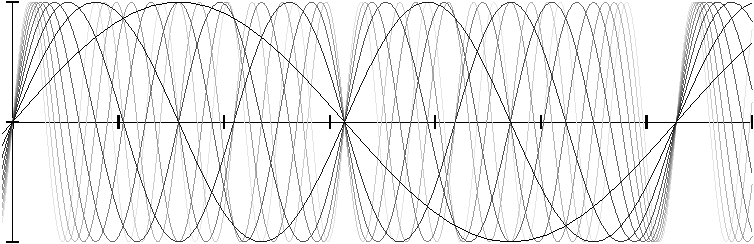
\includegraphics{figures/nonconvsinxn}
\caption{Graphs of $\sin(nx)$ for
$n=1,2,\ldots,10$, with higher $n$ in lighter gray.%
\label{fig:nonconvsinxn}}
\end{myfigureht}
\end{example}

Before we move to uniform convergence, let us reformulate pointwise
convergence in a different way.
We leave the proof to the reader---it is a simple application of the
definition of convergence of a sequence of real numbers.

\begin{prop} \label{ptwsconv:prop}
Let $f_n \colon S \to \R$ and $f \colon S \to \R$ be functions.
Then $\{ f_n \}_{n=1}^\infty$ converges pointwise to $f$ if and only if
for every $x \in S$, and every $\epsilon > 0$, there exists
an $N \in \N$ such that for all
$n \geq N$, we have
\begin{equation*}
\abs{f_n(x)-f(x)} < \epsilon .
\end{equation*}
\end{prop}

The key point here is that $N$ can depend on $x$, not just on
$\epsilon$.  That is, for each $x$ we can pick a different $N$.
If we could pick one $N$ for all $x$, we would have what is called
uniform convergence.

\subsection{Uniform convergence}

\begin{defn}
\index{uniform convergence}
Let $f_n \colon S \to \R$
and $f \colon S \to \R$
be functions.  The sequence $\{ f_n \}_{n=1}^\infty$
\emph{\myindex{converges uniformly}} to $f$ if for
every $\epsilon > 0$, there exists an $N \in \N$ such that 
for all $n \geq N$, we have
\begin{equation*}
\abs{f_n(x) - f(x)} < \epsilon \qquad \text{for all } x \in S.
\end{equation*}
\end{defn}
\begin{myfigureht}
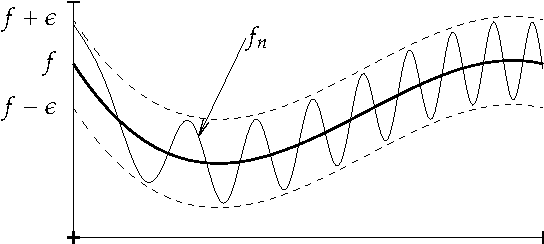
\includegraphics{figures/uniformconv}
\caption{In uniform convergence,
for $n \geq N$,
the functions $f_n$ are within a strip of $\pm\epsilon$ from $f$.%
\label{fig:uniformconv}}
\end{myfigureht}

In uniform convergence, $N$ cannot depend on $x$.  Given $\epsilon > 0$,
we must find an $N$ that works for all $x \in S$.  See
\figureref{fig:uniformconv} for an illustration.
Uniform convergence
implies pointwise convergence, and the proof follows by
\propref{ptwsconv:prop}:

\begin{prop}
Let $\{ f_n \}_{n=1}^\infty$ be a sequence of functions $f_n \colon S \to \R$.
If $\{ f_n \}_{n=1}^\infty$ converges
uniformly to $f \colon S \to \R$, then $\{ f_n \}_{n=1}^\infty$ converges pointwise to $f$.
\end{prop}

The converse does not hold.

\begin{example}
The functions $f_n(x) \coloneqq x^{2n}$ do not converge uniformly on $[-1,1]$,
even though they converge pointwise.  To see this, suppose for contradiction
that the convergence is uniform.  For $\epsilon \coloneqq \nicefrac{1}{2}$, there would have
to exist an $N$ such that $x^{2N} = \abs{x^{2N} - 0} < \nicefrac{1}{2}$ for all $x \in
(-1,1)$ (as $f_n(x)$ converges to 0 on $(-1,1)$).  But that means that
for every sequence $\{ x_k \}_{k=1}^\infty$ in $(-1,1)$ such that $\lim_{k\to\infty} x_k = 1$,
we have $x_k^{2N} < \nicefrac{1}{2}$ for all $k$.  On the other hand,
$x^{2N}$ is a continuous function of $x$ (it is a polynomial).  Therefore,
we obtain a contradiction
\begin{equation*}
1 = 1^{2N}  = \lim_{k\to\infty} x_k^{2N} \leq \nicefrac{1}{2} .
\end{equation*}

However, if we restrict our domain to $[-a,a]$ where $0 < a < 1$, then
$\{ f_n \}_{n=1}^\infty$ converges uniformly to 0 on $[-a,a]$.  Note that
$a^{2n} \to 0$ as $n \to \infty$.  Given $\epsilon > 0$,
pick $N \in \N$ such that
$a^{2n} < \epsilon$ for all $n \geq N$.
When $x \in [-a,a]$, we have
$\abs{x} \leq a$.  So
for all $n \geq N$ and all $x \in [-a,a]$,
\begin{equation*}
\abs{x^{2n}} = \abs{x}^{2n} \leq a^{2n} < \epsilon .
\end{equation*}
\end{example}

\subsection{Convergence in uniform norm}

For bounded functions, there is another more abstract way to 
think of uniform convergence.  To every bounded function we assign
a certain nonnegative number (called the uniform norm).  This number
measures the \myquote{distance} of the function from 0.  We can then
\myquote{measure}
how far two functions are from each other.  We then translate
a statement about uniform convergence into a statement about a certain
sequence of real numbers converging to zero.

\begin{defn} \label{def:unifnorm}
Let $f \colon S \to \R$ be a bounded function.  Define
\glsadd{not:uniformnorm}
\begin{equation*}
\snorm{f}_S \coloneqq
\sup \bigl\{ \abs{f(x)} : x \in S \bigr\} .
\end{equation*}
We call $\snorm{\cdot}_S$ the \emph{\myindex{uniform norm}}.
\end{defn}

The subscript is the set over which the supremum is taken.  So if $K \subset S$
then
\begin{equation*}
\snorm{f}_K =
\sup \bigl\{ \abs{f(x)} : x \in K \bigr\} .
\end{equation*}
Sometimes other notation\footnote{The notation nor terminology
is not completely standardized.  The norm is also called the
\emph{\myindex{sup norm}} or
\emph{\myindex{infinity norm}}, and in addition
to $\snorm{f}_u$ and $\snorm{f}_S$ it is sometimes written
as $\snorm{f}_{\infty}$ or $\snorm{f}_{\infty,S}$.}
is used, such as $\snorm{f}_u$.

\begin{prop}
A sequence of bounded functions $f_n \colon S \to \R$ converges
uniformly to $f \colon S \to \R$ if and only if
\begin{equation*}
\lim_{n\to\infty} \snorm{f_n - f}_S = 0 .
\end{equation*}
\end{prop}

\begin{proof}
First suppose 
$\lim_{n\to\infty} \norm{f_n - f}_S = 0$.  Let $\epsilon > 0$ be
given.  There exists an $N$ such that
for $n \geq N$, we have $\snorm{f_n - f}_S < \epsilon$.  As $\norm{f_n-f}_S$
is the supremum of $\abs{f_n(x)-f(x)}$, we see that for all $x \in S$,
we have $\abs{f_n(x)-f(x)} \leq \snorm{f_n - f}_S < \epsilon$.

On the other hand, suppose $\{ f_n \}_{n=1}^\infty$ converges uniformly to $f$.
Let $\epsilon > 0$ be given.  Then find $N$ such that 
$\abs{f_n(x)-f(x)} < \epsilon$ for all $x \in S$.
Taking the supremum we see that
$\snorm{f_n - f}_S \leq \epsilon$.  Hence $\lim_{n\to\infty} \snorm{f_n-f}_S = 0$.
\end{proof}

Sometimes it is said that \emph{$\{ f_n \}_{n=1}^\infty$ converges to $f$ in uniform norm}
\index{converges in uniform norm}
\index{uniform norm convergence}
instead of \emph{converges uniformly} if $\snorm{f_n-f}_S \to 0$.  The proposition
says that the two notions are the same thing.

\begin{example}
Let $f_n \colon [0,1] \to \R$ be defined by $f_n(x) \coloneqq \frac{nx+ \sin(nx^2)}{n}$.
We claim $\{ f_n \}_{n=1}^\infty$ converges uniformly to $f(x) \coloneqq x$.  Let us compute:
\begin{equation*}
\begin{split}
\norm{f_n-f}_{[0,1]}
& =
\sup \left\{ \abs{\frac{nx+ \sin(nx^2)}{n} - x} : x \in [0,1] \right\}
\\
& =
\sup \left\{ \frac{\abs{\sin(nx^2)}}{n} : x \in [0,1] \right\}
\\
& \leq
\sup \bigl\{ \nicefrac{1}{n} : x \in [0,1] \bigr\}
\\
& = \nicefrac{1}{n}.
\end{split}
\end{equation*}
\end{example}

Using the uniform norm, we define Cauchy sequences in a similar way
as we define Cauchy sequences of real numbers.

\begin{defn}
Let $f_n \colon S \to \R$ be bounded functions.
The sequence is \emph{\myindex{Cauchy in the uniform norm}}
or \emph{\myindex{uniformly Cauchy}}
if for every $\epsilon > 0$, there exists an $N \in \N$ such
that for all $m,k \geq N$,
\begin{equation*}
\norm{f_m-f_k}_S < \epsilon .
\end{equation*}
\end{defn}

\begin{prop} \label{prop:uniformcauchy}
Let $f_n \colon S \to \R$ be bounded functions.
Then $\{ f_n \}_{n=1}^\infty$ is Cauchy in the uniform norm if and only if
there exists an $f \colon S \to \R$ and $\{ f_n \}_{n=1}^\infty$ converges
uniformly to $f$.
\end{prop}

\begin{proof}
First suppose $\{ f_n \}_{n=1}^\infty$ is Cauchy in the uniform norm.
Let us define $f$.  Fix $x$.
The sequence $\bigl\{ f_n(x) \bigr\}_{n=1}^\infty$ is Cauchy because
\begin{equation*}
\abs{f_m(x)-f_k(x)}
\leq
\norm{f_m-f_k}_S .
\end{equation*}
Thus $\bigl\{ f_n(x) \bigr\}_{n=1}^\infty$ converges to some real number.  Define $f \colon S
\to \R$ by
\begin{equation*}
f(x) \coloneqq \lim_{n \to \infty} f_n(x) .
\end{equation*}
The sequence
$\{ f_n \}_{n=1}^\infty$ converges pointwise to $f$.  To show that the convergence
is uniform, let $\epsilon > 0$ be given.  Find an $N$ such that
for all $m, k \geq N$, we have
$\norm{f_m-f_k}_S < \nicefrac{\epsilon}{2}$.  In other words, for
all $x$, we have
$\abs{f_m(x)-f_k(x)} < \nicefrac{\epsilon}{2}$.  For any fixed $x$, take the limit
as $k$ goes to infinity.  Then $\abs{f_m(x)-f_k(x)}$
goes to $\abs{f_m(x)-f(x)}$.
Consequently for all $x$,
\begin{equation*}
\abs{f_m(x)-f(x)} \leq \nicefrac{\epsilon}{2} < \epsilon .
\end{equation*}
Hence, $\{ f_n \}_{n=1}^\infty$ converges uniformly.

Next, we prove the other direction.
Suppose $\{ f_n \}_{n=1}^\infty$ converges uniformly to
$f$.  Given $\epsilon > 0$, find $N$ such that for all $n \geq N$,
we have $\abs{f_n(x)-f(x)} < \nicefrac{\epsilon}{4}$ for all $x \in S$.
Therefore, for all $m, k \geq N$ and all $x$,
\begin{equation*}
\abs{f_m(x)-f_k(x)} = 
\abs{f_m(x)-f(x)+f(x)-f_k(x)} \leq
\abs{f_m(x)-f(x)}+\abs{f(x)-f_k(x)} < \nicefrac{\epsilon}{4} +
\nicefrac{\epsilon}{4} .
\end{equation*}
Take supremum over all $x$ to obtain
\begin{equation*}
\norm{f_m-f_k}_S \leq \nicefrac{\epsilon}{2} < \epsilon .  \qedhere
\end{equation*}
\end{proof}

\subsection{Exercises}

\begin{exercise}
Let $f$ and $g$ be bounded functions on $[a,b]$.  Prove 
\begin{equation*}
\norm{f+g}_{[a,b]} \leq \norm{f}_{[a,b]} + \norm{g}_{[a,b]} .
\end{equation*}
\end{exercise}

\begin{exercise}
\leavevmode
\begin{enumerate}[a)]
\item
Find the pointwise limit $\dfrac{e^{x/n}}{n}$ for $x \in \R$.
\item
Is the limit uniform on $\R$?
\item
Is the limit uniform on $[0,1]$?
\end{enumerate}
\end{exercise}

\begin{exercise}
Suppose $f_n \colon S \to \R$ are functions that converge uniformly
to $f \colon S \to \R$.  Suppose $A \subset S$.  Show that
the sequence of restrictions $\{ f_n|_A \}_{n=1}^\infty$ converges uniformly to $f|_A$.
\end{exercise}

\begin{exercise}
Suppose $\{ f_n \}_{n=1}^\infty$ and $\{ g_n \}_{n=1}^\infty$ defined on some set $A$ converge to
$f$ and $g$ respectively pointwise.  Show that $\{ f_n+g_n \}_{n=1}^\infty$ converges
pointwise to $f+g$.
\end{exercise}

\begin{exercise}
Suppose $\{ f_n \}_{n=1}^\infty$ and $\{ g_n \}_{n=1}^\infty$ defined on some set $A$ converge to
$f$ and $g$ respectively uniformly on $A$.
Show that $\{ f_n+g_n \}_{n=1}^\infty$
converges uniformly to $f+g$ on $A$.
\end{exercise}

\begin{exercise}
Find an example of a sequence of functions $\{ f_n \}_{n=1}^\infty$ and $\{
g_n \}_{n=1}^\infty$
that converge uniformly to some $f$ and $g$ on some set $A$, but such that
$\{ f_ng_n \}_{n=1}^\infty$ (the multiple) does not converge uniformly to $fg$ on $A$.
Hint: Let $A \coloneqq \R$, let $f(x)\coloneqq g(x) \coloneqq x$.  You can even pick $f_n = g_n$.
\end{exercise}

\begin{exercise}
Suppose there exists a sequence of functions $\{ g_n \}_{n=1}^\infty$ uniformly
converging to $0$ on $A$.  Now suppose we have a sequence of functions
$\{ f_n \}_{n=1}^\infty$ and a function $f$ on $A$ such that
\begin{equation*}
\abs{f_n(x) - f(x)} \leq g_n(x) 
\end{equation*}
for all $x \in A$.  Show that $\{ f_n \}_{n=1}^\infty$ converges uniformly to $f$ on $A$.
\end{exercise}

\begin{exercise}
Let $\{ f_n \}_{n=1}^\infty$, $\{ g_n \}_{n=1}^\infty$ and
$\{ h_n \}_{n=1}^\infty$ be sequences of functions on
$[a,b]$.  Suppose $\{ f_n \}_{n=1}^\infty$ and $\{ h_n \}_{n=1}^\infty$ converge uniformly to some function
$f \colon [a,b] \to \R$ and suppose $f_n(x) \leq g_n(x) \leq h_n(x)$
for all $x \in [a,b]$.  Show that $\{ g_n \}_{n=1}^\infty$ converges uniformly to $f$.
\end{exercise}

\begin{exercise}
Let $f_n \colon [0,1] \to \R$ be a sequence of increasing functions (that
is, $f_n(x) \geq f_n(y)$ whenever $x \geq y$).  Suppose $f_n(0) = 0$
and $\lim\limits_{n \to \infty} f_n(1) = 0$.  Show that
$\{ f_n \}_{n=1}^\infty$
converges uniformly to $0$.
\end{exercise}

\begin{exercise}
Let $\{f_n\}_{n=1}^\infty$ be a sequence of functions defined on $[0,1]$.
Suppose there exists a sequence of distinct numbers $x_n \in [0,1]$ such that
\begin{equation*}
f_n(x_n) = 1 .
\end{equation*}
Prove or disprove the following statements:
\begin{enumerate}[a)]
\item
True or false: There exists $\{ f_n \}_{n=1}^\infty$ as above that converges to $0$
pointwise.
\item
True or false: There exists $\{ f_n \}_{n=1}^\infty$ as above that converges to $0$
uniformly on $[0,1]$.
\end{enumerate}
\end{exercise}

\begin{exercise}
Fix a continuous $h \colon [a,b] \to \R$.
Let $f(x) \coloneqq h(x)$ for $x \in [a,b]$,
$f(x) \coloneqq h(a)$ for $x < a$ and $f(x) \coloneqq h(b)$ for all $x > b$.  First show
that $f \colon \R \to \R$ is continuous.
Now let $f_n$ be
the function $g$ from \exerciseref{exercise:smoothingout} with
$\epsilon = \nicefrac{1}{n}$, defined on the interval $[a,b]$.  That is,
\begin{equation*}
f_n(x) \coloneqq \frac{n}{2} \int_{x-1/n}^{x+1/n} f .
\end{equation*}
Show that $\{ f_n \}_{n=1}^\infty$ converges uniformly to $h$ on $[a,b]$.
\end{exercise}


\begin{exercise}
Prove that
if a sequence of functions $f_n \colon S \to \R$
converge uniformly to a bounded function $f \colon S \to \R$,
then there exists an $N$ such that for all $n \geq N$, the $f_n$
are bounded.
\end{exercise}

\begin{exercise}
Suppose there is a single constant $B$ and
a sequence of functions
$f_n \colon S \to \R$ that are bounded by $B$,
that is $\abs{f_n(x)} \leq B$ for all $x \in S$.
Suppose that $\{ f_n \}_{n=1}^\infty$ converges pointwise
to $f \colon S \to \R$.
Prove that $f$ is bounded.
\end{exercise}

\begin{exercise}[requires \sectionref{sec:moreonseries}]
In \exampleref{example:geomsumptconv} we saw
$\sum_{k=0}^\infty x^k$ converges pointwise to $\frac{1}{1-x}$ on
$(-1,1)$.
\begin{enumerate}[a)]
\item
Show that whenever $0 \leq c < 1$, the series
$\sum_{k=0}^\infty x^k$ converges uniformly on $[-c,c]$.
\item
Show that the series $\sum_{k=0}^\infty x^k$ does not converge uniformly
on $(-1,1)$.
\end{enumerate}
\end{exercise}

%%%%%%%%%%%%%%%%%%%%%%%%%%%%%%%%%%%%%%%%%%%%%%%%%%%%%%%%%%%%%%%%%%%%%%%%%%%%%%

\sectionnewpage
\section{Interchange of limits}
\label{sec:liminter}

\sectionnotes{1--2.5 lectures,
subsections on derivatives and power series (which
requires \sectionref{sec:moreonseries}) optional.}

Large parts of modern analysis deal mainly with the question of the
interchange of two limiting operations.  When
we have a chain of two limits, we cannot always just swap the limits.
For instance,
\begin{equation*}
0 = 
\lim_{n\to\infty}
\left(
\lim_{k\to\infty}
\frac{n}{n + k}
\right)
\not=
\lim_{k\to\infty}
\left(
\lim_{n\to\infty}
\frac{n}{n + k}
\right)
= 1 .
\end{equation*}

When talking about sequences of functions, interchange of limits comes up
quite often.  We look at several instances: continuity of the limit, the
integral of the limit, the derivative of the limit, and the convergence of
power series.

\subsection{Continuity of the limit}

If we have a sequence $\{ f_n \}_{n=1}^\infty$ of continuous functions, is the limit continuous?
Suppose $f$ is the (pointwise) limit of $\{ f_n \}_{n=1}^\infty$.
If $\lim_{k\to\infty} x_k = x$,
we are interested in the following
interchange of limits, where the equality to prove
is marked with a question mark.  Equality is not always true, in fact, the limits to the left
of the question mark might not even exist.
\begin{equation*}
\lim_{k \to \infty} 
f(x_k)
=
\lim_{k \to \infty} 
\Bigl(
\lim_{n \to \infty} f_n(x_k)
\Bigr)
\overset{?}{=}
\lim_{n \to \infty}
\Bigl(
\lim_{k \to \infty} 
f_n(x_k)
\Bigr)
=
\lim_{n \to \infty}
f_n(x)
=
f(x) .
\end{equation*}
We wish to find conditions on the sequence $\{ f_n \}_{n=1}^\infty$
so that the equation above holds.
If we only require pointwise convergence, then the limit
of a sequence of functions need not be continuous, and the equation above
need not hold.

\begin{example}
Define $f_n \colon [0,1] \to \R$ as
\begin{equation*}
f_n(x) \coloneqq
\begin{cases}
1-nx &  \text{if } x < \nicefrac{1}{n},\\
0 &  \text{if } x \geq \nicefrac{1}{n}.
\end{cases}
\end{equation*}
See \figureref{contconvcntr:fig}.

\begin{myfigureht}
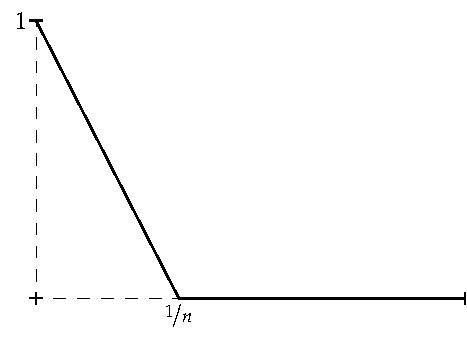
\includegraphics{figures/contconvcntr}
\caption{Graph of $f_n(x)$.%
\label{contconvcntr:fig}}
\end{myfigureht}

Each function $f_n$ is continuous.
Fix an $x \in (0,1]$.  If $n \geq \nicefrac{1}{x}$,
then $x \geq \nicefrac{1}{n}$.  Therefore for $n \geq \nicefrac{1}{x}$,
we have $f_n(x) = 0$, and so
\begin{equation*}
\lim_{n \to \infty} f_n(x) = 0.
\end{equation*}
On the other hand, if $x=0$, then
\begin{equation*}
\lim_{n \to \infty} f_n(0) = 
\lim_{n \to \infty} 1 = 1.
\end{equation*}
Thus the pointwise limit of $f_n$ is the function
$f \colon [0,1] \to \R$ defined by
\begin{equation*}
f(x) \coloneqq
\begin{cases}
1 &  \text{if } x = 0,\\
0 &  \text{if } x > 0.
\end{cases}
\end{equation*}
The function $f$ is not continuous at 0.
\end{example}

If we, however, require the convergence to be uniform, the limits can
be interchanged.

\begin{thm}
Suppose $S \subset \R$.
Let $\{ f_n \}_{n=1}^\infty$ be 
a sequence of continuous functions $f_n \colon S \to \R$ converging
uniformly to  $f \colon S \to \R$.  Then $f$ is continuous.
\end{thm}

\begin{proof}
Let $x \in S$ be fixed.  Let $\{ x_n \}_{n=1}^\infty$ be a sequence in $S$
converging to $x$.

Let $\epsilon > 0$ be given.
As $\{ f_k \}_{k=1}^\infty$ converges uniformly to $f$, we find a $k \in \N$ such that
\begin{equation*}
\abs{f_k(y)-f(y)} < \nicefrac{\epsilon}{3}
\end{equation*}
for all $y \in S$.  As $f_k$ is continuous at $x$,
we find an $N \in \N$ such that for all $m \geq N$,
\begin{equation*}
\abs{f_k(x_m)-f_k(x)} < \nicefrac{\epsilon}{3} .
\end{equation*}
Thus for all
$m \geq N$,
\begin{equation*}
\begin{split}
\abs{f(x_m)-f(x)}
& =
\abs{f(x_m)-f_k(x_m)+f_k(x_m)-f_k(x)+f_k(x)-f(x)}
\\
& \leq
\abs{f(x_m)-f_k(x_m)}+
\abs{f_k(x_m)-f_k(x)}+
\abs{f_k(x)-f(x)}
\\
& <
\nicefrac{\epsilon}{3} +
\nicefrac{\epsilon}{3} +
\nicefrac{\epsilon}{3} = \epsilon .
\end{split}
\end{equation*}
Therefore, $\bigl\{ f(x_m) \bigr\}_{m=1}^\infty$ converges to $f(x)$ and $f$ is continuous at
$x$.  As $x$ was arbitrary, $f$ is continuous everywhere.
\end{proof}

\subsection{Integral of the limit}

Again, if we simply require pointwise convergence, then the integral
of a limit of a sequence of functions need not be equal to the limit
of the integrals.

\begin{example}
Define $f_n \colon [0,1] \to \R$ as
\begin{equation*}
f_n(x) \coloneqq
\begin{cases}
0 &  \text{if } x = 0,\\
n-n^2x &  \text{if } 0 < x < \nicefrac{1}{n},\\
0 &  \text{if } x \geq \nicefrac{1}{n}.
\end{cases}
\avoidbreak
\end{equation*}
See \figureref{intconvcntr:fig}.

\begin{myfigureht}
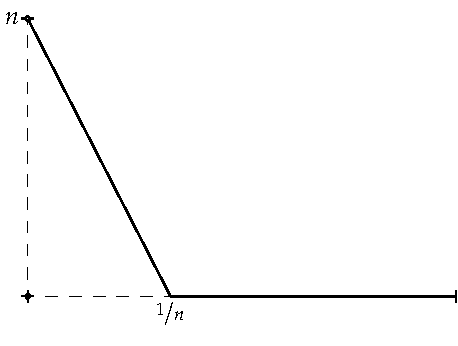
\includegraphics{figures/intconvcntr}
\caption{Graph of $f_n(x)$.%
\label{intconvcntr:fig}}
\end{myfigureht}

Each $f_n$ is Riemann integrable (it is continuous on $(0,1]$ and bounded),
and the fundamental theorem of calculus says that
\begin{equation*}
\int_0^1 f_n =
\int_0^{\nicefrac{1}{n}} (n-n^2x)\,dx = \nicefrac{1}{2} .
\end{equation*}
Let us compute the pointwise limit of $\{ f_n \}_{n=1}^\infty$.
Fix an $x \in (0,1]$.  For $n \geq \nicefrac{1}{x}$,
we have $x \geq \nicefrac{1}{n}$ and so $f_n(x) = 0$.  Therefore,
\begin{equation*}
\lim_{n \to \infty} f_n(x) = 0.
\end{equation*}
We also have $f_n(0) = 0$ for all $n$.  Therefore, the pointwise
limit of $\{ f_n \}_{n=1}^\infty$ is the zero function.  Thus
\begin{equation*}
\nicefrac{1}{2} =
\lim_{n\to\infty}
\int_0^1 f_n (x)\,dx
\not=
\int_0^1
\left(
\lim_{n\to\infty}
f_n(x)\right)\,dx
=
\int_0^1 0\,dx = 0 .
\end{equation*}
\end{example}

But if we require the convergence to be uniform, the limits can
be interchanged.\footnote{Weaker conditions
are sufficient for this kind of theorem, but to prove such a generalization requires
more sophisticated machinery than we cover here: the Lebesgue integral.
In particular, the theorem holds with pointwise
convergence as long as $f$ is integrable and there is an $M$ such that
$\snorm{f_n}_{[a,b]} \leq M$ for all $n$.}

\begin{thm} \label{integralinterchange:thm}
Let $\{ f_n \}_{n=1}^\infty$ be a sequence of Riemann integrable
functions
$f_n \colon [a,b] \to \R$
converging uniformly to $f \colon [a,b]
\to \R$.  Then $f$ is Riemann integrable, and
\begin{equation*}
\int_a^b f = \lim_{n\to\infty} \int_a^b f_n .
\end{equation*}
\end{thm}

\begin{proof}
Let $\epsilon > 0$ be given.
As $f_n$ goes to $f$ uniformly, we find an $M \in \N$ such that
for all $n \geq M$, we have 
$\abs{f_n(x)-f(x)} < \frac{\epsilon}{2(b-a)}$ for all $x \in [a,b]$.
In particular, by reverse triangle inequality,
$\abs{f(x)} < \frac{\epsilon}{2(b-a)} + \abs{f_n(x)}$ for all $x$.
Hence $f$ is bounded,
as $f_n$ is bounded.
Note that $f_n$ is integrable and compute
\begin{equation*}
\begin{split}
\overline{\int_a^b} f
-
\underline{\int_a^b} f
& =
\overline{\int_a^b} \bigl( f(x) - f_n(x) + f_n(x) \bigr)\,dx
-
\underline{\int_a^b} \bigl( f(x) - f_n(x) + f_n(x) \bigr)\,dx
\\
& \leq
\overline{\int_a^b} \bigl( f(x) - f_n(x) \bigr)\,dx +  \overline{\int_a^b} f_n(x) \,dx
-
\underline{\int_a^b} \bigl( f(x) - f_n(x) \bigr)\,dx -  \underline{\int_a^b} f_n(x) \,dx
\\
& =
\overline{\int_a^b} \bigl( f(x) - f_n(x) \bigr)\,dx +  \int_a^b f_n(x) \,dx
-
\underline{\int_a^b} \bigl( f(x) - f_n(x) \bigr)\,dx -  \int_a^b f_n(x) \,dx
\\
& =
\overline{\int_a^b} \bigl( f(x) - f_n(x) \bigr)\,dx
-
\underline{\int_a^b} \bigl( f(x) - f_n(x) \bigr)\,dx
\\
& \leq
\frac{\epsilon}{2(b-a)} (b-a) + 
\frac{\epsilon}{2(b-a)} (b-a) = \epsilon .
\end{split}
\end{equation*}
The first inequality is \propref{prop:upperlowerlinineq}.
The second inequality follows from \propref{intulbound:prop} and 
the fact that for all $x \in [a,b]$, we have
$\frac{-\epsilon}{2(b-a)} < f(x)-f_n(x) < \frac{\epsilon}{2(b-a)}$.
As $\epsilon > 0$ was arbitrary, $f$ is Riemann integrable.

Finally, we compute $\int_a^b f$.  We apply \propref{intbound:prop}
in the calculation.  Again, for all $n \geq M$ (where $M$ is the same as above),
\begin{equation*}
\begin{split}
\abs{\int_a^b f - \int_a^b f_n} & = 
\abs{ \int_a^b \bigl(f(x) - f_n(x)\bigr)\,dx}
\\
& \leq
\frac{\epsilon}{2(b-a)} (b-a) = \frac{\epsilon}{2} < \epsilon .
\end{split}
\end{equation*}
Therefore, $\bigl\{ \int_a^b f_n \bigr\}_{n=1}^\infty$ converges to $\int_a^b f$.
\end{proof}

\begin{example}
Suppose we wish to compute
\begin{equation*}
\lim_{n\to\infty} \int_0^1 \frac{nx+ \sin(nx^2)}{n} \,dx .
\end{equation*}
It is impossible to compute the integrals for any particular $n$ using 
calculus as $\sin(nx^2)$ has no closed-form antiderivative.  However,
we can compute the limit.
We have shown before that $\frac{nx+ \sin(nx^2)}{n}$ converges uniformly
on $[0,1]$ to $x$.
By \thmref{integralinterchange:thm}, the limit exists and
\begin{equation*}
\lim_{n\to\infty} \int_0^1 \frac{nx+ \sin(nx^2)}{n} \,dx
=
\int_0^1
x \,dx = \nicefrac{1}{2} .
\end{equation*}
\end{example}

\begin{example}
If convergence is only pointwise, the limit need not even be Riemann
integrable.  On $[0,1]$ define
\begin{equation*}
f_n(x) \coloneqq
\begin{cases}
1 & \text{if } x = \nicefrac{p}{q} \text{ in lowest terms and } q \leq n, \\
0 & \text{otherwise.}
\end{cases}
\end{equation*}
The function $f_n$ differs from the zero function at finitely many points;
there are only finitely many fractions in $[0,1]$ with denominator less than
or equal to $n$.   So $f_n$ is integrable and $\int_0^1 f_n = \int_0^1 0 =
0$.  It is an easy exercise to show that $\{ f_n \}_{n=1}^\infty$ converges pointwise to the
\myindex{Dirichlet function}
\begin{equation*}
f(x) \coloneqq
\begin{cases}
1 & \text{if } x \in \Q, \\
0 & \text{otherwise,}
\end{cases}
\end{equation*}
which is not Riemann integrable.
\end{example}

\begin{example}
In fact, if the convergence is only pointwise, the limit of bounded
functions is not even necessarily bounded.
Define $f_n \colon [0,1] \to \R$ by
\begin{equation*}
f_n(x) \coloneqq
\begin{cases}
0 & \text{if } x < \nicefrac{1}{n},\\
\nicefrac{1}{x} & \text{else.}
\end{cases}
\end{equation*}
For every $n$ we get that $\abs{f_n(x)} \leq n$ for all $x \in [0,1]$ so the
functions are bounded.  However $f_n$ converge pointwise to
\begin{equation*}
f(x) \coloneqq
\begin{cases}
0 & \text{if } x = 0,\\
\nicefrac{1}{x} & \text{else,}
\end{cases}
\end{equation*}
which is unbounded.
\end{example}

\subsection{Derivative of the limit}

While uniform convergence is enough to swap limits with integrals, it is not,
however, enough to swap limits with derivatives, unless you also have
uniform convergence of the derivatives themselves.

\begin{example}
Let $f_n(x) \coloneqq \frac{\sin(nx)}{n}$.  Then $f_n$ converges uniformly to
0.  See \figureref{fig:conv1nsinxn}.
The derivative of the limit is 0.  But $f_n'(x) = \cos(nx)$, which
does not converge even pointwise, for
example $f_n'(\pi) = {(-1)}^n$.  Furthermore,
$f_n'(0) = 1$ for all $n$, which does converge, but not to $0$.
\begin{myfigureht}
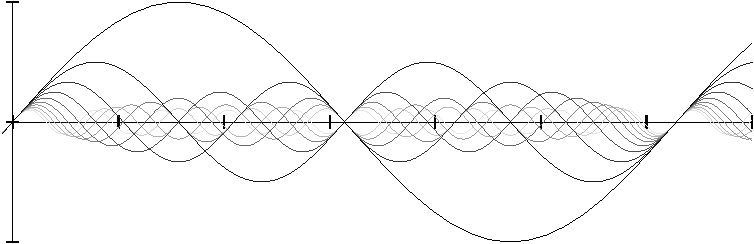
\includegraphics{figures/conv1nsinxn}
\caption{Graphs of $\frac{\sin(nx)}{n}$ for
$n=1,2,\ldots,10$, with higher $n$ in lighter gray.%
\label{fig:conv1nsinxn}}
\end{myfigureht}
\end{example}

\begin{example} \label{exercise:badconvergenceder}
Let $f_n(x) \coloneqq \frac{1}{1+nx^2}$.
If $x \not= 0$, then $\lim_{n \to \infty} f_n(x) = 0$,
but $\lim_{n \to \infty} f_n(0) = 1$.
Hence, $\{ f_n \}_{n=1}^\infty$ converges pointwise to a function that is not continuous
at $0$.
We compute
\begin{equation*}
f_n'(x) %= \frac{d}{dx} \frac{1}{1+n x^2}
= \frac{-2 n x}{(1+ n x^2)^2} .
\end{equation*}
For every $x$, $\lim_{n\to\infty} f_n'(x) = 0$, so the derivatives
converge pointwise to 0,
but the reader can check that the convergence is not uniform on any
interval containing $0$.
The limit of $f_n$ is not differentiable at $0$---it is not even
continuous at $0$.
\end{example}

See the exercises for more examples.  Using 
the fundamental theorem of calculus, we find an answer for continuously
differentiable functions.  The following theorem is true even if 
we do not assume continuity of the derivatives, but the proof is more
difficult.

\begin{thm} \label{thm:dersconverge}
Let $I$ be a bounded interval and let
$f_n \colon I \to \R$ be continuously differentiable functions.
Suppose $\{ f_n' \}_{n=1}^\infty$ converges uniformly to $g \colon I \to \R$,
and suppose $\bigl\{ f_n(c) \bigr\}_{n=1}^\infty$ is a
convergent sequence for some $c \in I$.  Then $\{ f_n \}_{n=1}^\infty$ converges uniformly to 
a continuously differentiable function $f \colon I \to \R$, and $f' = g$.
\end{thm}

\begin{proof}
Define $f(c) \coloneqq \lim_{n\to \infty} f_n(c)$.
As $f_n'$ are continuous and hence Riemann integrable,
then
via the fundamental theorem of calculus, we find that for $x \in I$,
\begin{equation*}
f_n(x) = f_n(c) + \int_c^x f_n' .
\end{equation*}
As $\{ f_n' \}_{n=1}^\infty$ converges uniformly on $I$, it converges uniformly
on $[c,x]$ (or $[x,c]$ if $x < c$).
Thus, the limit as $n \to \infty$ on the right-hand side exists.
Define $f$ at the remaining points (where $x\neq c$) by this limit:
\begin{equation*}
f(x) \coloneqq
\lim_{n\to\infty} f_n(c) + \lim_{n\to\infty} \int_c^x f_n'
=
f(c) + \int_c^x g .
\end{equation*}
The function $g$ is continuous, being the uniform limit of continuous
functions.  Hence $f$ is differentiable and $f'(x) = g(x)$ for all $x \in I$
by the second form of the fundamental theorem.

It remains to prove
uniform convergence.
Suppose $I$ has a lower bound $a$ and upper bound $b$.
Let $\epsilon > 0$ be given.  Take $M$
such that for all $n \geq M$, we have
$\abs{f(c)-f_n(c)} < \nicefrac{\epsilon}{2}$
and
$\abs{g(x)-f_n'(x)} < \frac{\epsilon}{2(b-a)}$
for all $x \in I$.  Then
\begin{equation*}
\begin{split}
\abs{f(x) - f_n(x)} & =
\abs{\left(f(c) + \int_c^x g\right) - \left( f_n(c) + \int_c^x f_n' \right)}
\\
& \leq
\abs{f(c) - f_n(c)} + \abs{\int_c^x g - \int_c^x f_n'}
\\
& =
\abs{f(c) - f_n(c)} + \abs{\int_c^x \bigl(g(s) - f_n'(s)\bigr) \, ds}
\\
& <
\frac{\epsilon}{2}
+
\frac{\epsilon}{2(b-a)}
(b-a)
=\epsilon. \qedhere
\end{split}
\end{equation*}
\end{proof}

The proof goes through without boundedness of $I$, except for the
uniform convergence of $f_n$ to $f$.  As an example suppose $I = \R$ and let
$f_n(x) \coloneqq \nicefrac{x}{n}$.  Then $f_n'(x)=\nicefrac{1}{n}$, which
converges uniformly to $0$.  However, $\{f_n\}_{n=1}^\infty$ converges to 0 only pointwise.

\subsection{Convergence of power series}

In \sectionref{sec:moreonseries} we saw that a power series converges
absolutely inside its radius of convergence, so it converges pointwise.
Let us show that it (and all its derivatives) also converges uniformly.
This fact allows us to
swap several types of limits.  Not only is the limit continuous,
we can
integrate and even differentiate convergent power series term by term.

\begin{prop}
Let $\sum_{n=0}^\infty c_n {(x-a)}^n$ be a convergent power series with a radius
of convergence $\rho$, where $0 < \rho \leq \infty$.
Then the series converges uniformly
in $[a-r,a+r]$ whenever $0 < r < \rho$.

In particular, the series converges (pointwise) to a continuous function
on $(a-\rho,a+\rho)$ if $\rho < \infty$, or on $\R$ if $\rho = \infty$.
\end{prop}

\begin{proof}
Let $I \coloneqq (a-\rho,a+\rho)$ if $\rho < \infty$,
or let $I \coloneqq \R$ if $\rho= \infty$.
Take $0 < r < \rho$.
The series converges absolutely for every $x \in I$,
in particular if $x = a+r$.
So $\sum_{n=0}^\infty \abs{c_n} r^n$ converges.
Given $\epsilon >0$, find $M$ such that for all $k \geq M$,
\begin{equation*}
\sum_{n=k+1}^\infty \abs{c_n} {r}^n < \epsilon .
\end{equation*}
For all $x \in [a-r,a+r]$ and all $m > k$,
\begin{multline*}
\abs{\sum_{n=0}^m c_n {(x-a)}^n - 
\sum_{n=0}^k c_n {(x-a)}^n}
=
\abs{\sum_{n=k+1}^m c_n {(x-a)}^n}
\\
\leq
\sum_{n=k+1}^m \abs{c_n} {\abs{x-a}}^n
\leq
\sum_{n=k+1}^m \abs{c_n} {r}^n
\leq
\sum_{n=k+1}^\infty \abs{c_n} {r}^n
<\epsilon.
\end{multline*}
The partial sums are therefore uniformly Cauchy on $[a-r,a+r]$ and
hence converge uniformly on that set.

Moreover, the partial sums are polynomials, which are
continuous, and so their uniform limit on $[a-r,a+r]$
is a continuous function.
As $r < \rho$ was arbitrary, the limit function
is continuous on all of $I$.
\end{proof}

As we said, we will show that
power series can be differentiated and integrated
term by term.  The 
differentiated or integrated series is again a power series,
and we will show it has the same radius of convergence.
Therefore, 
any power series defines an infinitely differentiable function.

We first prove that we can antidifferentiate, as integration only needs
uniform limits.

\begin{cor}
Let $\sum_{n=0}^\infty c_n {(x-a)}^n$ be a convergent power series with a radius
of convergence $0 < \rho \leq \infty$.
Let $I \coloneqq (a-\rho,a+\rho)$ if $\rho < \infty$
or $I \coloneqq \R$ if $\rho= \infty$.  Let $f \colon I \to \R$ be the limit.
Then
\begin{equation*}
\int_a^x f = \sum_{n=1}^\infty \frac{c_{n-1}}{n} {(x-a)}^{n} ,
\end{equation*}
where the radius of convergence of this series is at least $\rho$.
\end{cor}

\begin{proof}
Take $0 < r < \rho$.
The partial sums $\sum_{n=0}^k c_n {(x-a)}^n$ converge uniformly on $[a-r,a+r]$.
For every fixed $x \in [a-r,a+r]$, the convergence is also uniform
on $[a,x]$ (or $[x,a]$ if $x < a$).
Hence,
\begin{equation*}
\int_a^x f =
\int_a^x \lim_{k\to\infty} \sum_{n=0}^k c_n {(s-a)}^n \, ds
=
\lim_{k\to\infty}
\int_a^x \sum_{n=0}^k c_n {(s-a)}^n \, ds
=
\lim_{k\to\infty}
\sum_{n=1}^{k+1} \frac{c_{n-1}}{n} {(x-a)}^{n} . \qedhere
\end{equation*}
\end{proof}


\begin{cor} \label{cor:differentiatepowerser}
Let $\sum_{n=0}^\infty c_n {(x-a)}^n$ be a convergent power series with a radius
of convergence $0 < \rho \leq \infty$.
Let $I \coloneqq (a-\rho,a+\rho)$ if $\rho < \infty$
or $I \coloneqq \R$ if $\rho= \infty$.  Let $f \colon I \to \R$ be the limit.
Then $f$ is a differentiable function, and
\begin{equation*}
f'(x) = \sum_{n=0}^\infty (n+1) c_{n+1} {(x-a)}^{n} ,
\end{equation*}
where the radius of convergence of this series is $\rho$.
\end{cor}

\begin{proof}
Take $0 < r < \rho$.
The series converges uniformly on
$[a-r,a+r]$,
but we need uniform convergence of the derivative.
Let
\begin{equation*}
R \coloneqq \limsup_{n \to \infty} \abs{c_n}^{1/n} .
\end{equation*}
As the series is convergent $R < \infty$, and
the radius of convergence is $\nicefrac{1}{R}$ (or $\infty$ if $R=0$).

Let $\epsilon > 0$ be given.  In \exampleref{example:nto1overn},
we saw $\lim_{n\to\infty} n^{1/n} = 1$.
Hence there exists an $N$ such that for all $n \geq N$, we have
$n^{1/n} < 1+\epsilon$.
So
\begin{equation*}
R = 
\limsup_{n \to \infty}
\abs{c_n}^{1/n}
\leq
\limsup_{n \to \infty}
\abs{n c_n}^{1/n}
\leq
(1+\epsilon)
\limsup_{n \to \infty}
\abs{c_n}^{1/n}
=
(1+\epsilon)R .
\end{equation*}
As $\epsilon$ was arbitrary, $\limsup_{n \to \infty} \abs{n c_n}^{1/n} = R$.
Therefore, $\sum_{n=1}^\infty n c_{n} {(x-a)}^{n}$ has radius of
convergence $\rho$.  By dividing by $(x-a)$, we find
$\sum_{n=0}^\infty (n+1) c_{n+1} {(x-a)}^{n}$ has radius of convergence
$\rho$ as well.

Consequently, the partial sums 
$\sum_{n=0}^k (n+1) c_{n+1} {(x-a)}^{n}$,
which are derivatives of the partial sums
$\sum_{n=0}^{k+1} c_{n} {(x-a)}^{n}$,
converge uniformly on $[a-r,a+r]$.  Furthermore,
the series clearly converges at $x=a$.
We may thus apply \thmref{thm:dersconverge}, and
we are done as $r < \rho$ was arbitrary.
\end{proof}

\begin{example} \label{example:exponentialbypowerseries}
We could have used this result to define the exponential function.  That is,
the power series
\begin{equation*}
f(x) \coloneqq \sum_{n=0}^\infty \frac{x^n}{n!}
\end{equation*}
has radius of convergence $\rho=\infty$.  Furthermore,
$f(0) = 1$, and by differentiating
term by term, we find that $f'(x) = f(x)$.
\end{example}

\begin{example}
The series
\begin{equation*}
\sum_{n=1}^\infty n x^n
\end{equation*}
converges to $\frac{x}{{(1-x)}^2}$ on $(-1,1)$.

Proof:
On $(-1,1)$, $\sum_{n=0}^\infty x^n$ converges to
$\frac{1}{1-x}$.  The derivative $\sum_{n=1}^\infty n x^{n-1}$ then converges
on the same interval to $\frac{1}{{(1-x)}^2}$.  Multiplying by $x$
obtains the result.
\end{example}

\subsection{Exercises}

\begin{exercise}
%While uniform convergence preserves continuity, it does not preserve
%differentiability.
Find an explicit example of a sequence of
differentiable functions on $[-1,1]$ that converge uniformly to
a function $f$ such that $f$ is not differentiable.
Hint:
There are many possibilities,
simplest is perhaps to combine $\abs{x}$ and $\frac{n}{2}x^2 +
\frac{1}{2n}$, another is to
consider $\sqrt{x^2+{(\nicefrac{1}{n})}^2}$.  Show that these functions are differentiable,
converge uniformly, and then show that the limit is not differentiable.
\end{exercise}

\begin{exercise}
Let $f_n(x) \coloneqq \frac{x^n}{n}$.  Show that $\{ f_n \}_{n=1}^\infty$ converges uniformly to
a differentiable function $f$ on $[0,1]$ (find $f$).  However, show that
$f'(1) \not= \lim\limits_{n\to\infty} f_n'(1)$.
\end{exercise}

%\begin{exnote}
%Note: The previous two exercises show that
%we cannot simply swap limits with derivatives, even if the convergence is
%uniform.  See also \exerciseref{c1uniflim:exercise} below.
%\end{exnote}
%
\begin{exercise}
Let $f \colon [0,1] \to \R$ be a Riemann integrable (hence bounded)
function.  Find
$\displaystyle \lim_{n\to\infty} \int_0^1 \frac{f(x)}{n} \,dx$.
\end{exercise}

\begin{exercise}
Show
$\displaystyle \lim_{n\to\infty} \int_1^2 e^{-nx^2} \,dx = 0$.  Feel free to
use
what you know about the exponential function from calculus.
\end{exercise}

\begin{exercise}
Find an example of a sequence of continuous functions on $(0,1)$ that converges 
pointwise to a continuous function on $(0,1)$, but the convergence is not
uniform.
\end{exercise}

\begin{exnote}
Note: In the previous exercise, $(0,1)$ was picked for simplicity.  For a
more challenging exercise, replace $(0,1)$ with $[0,1]$.
\end{exnote}

\begin{exercise}
True/False; prove or find a counterexample to the following statement:
If $\{ f_n \}_{n=1}^\infty$ is a sequence of everywhere discontinuous functions on $[0,1]$
that converge uniformly to a function $f$, then $f$ is everywhere
discontinuous.
\end{exercise}

\begin{exercise} \label{c1uniflim:exercise}
For a continuously differentiable function $f \colon [a,b] \to \R$, define
\begin{equation*}
\norm{f}_{C^1} \coloneqq \norm{f}_{[a,b]} + \norm{f'}_{[a,b]} .
\end{equation*}
Suppose $\{ f_n \}_{n=1}^\infty$ is a sequence of continuously differentiable
functions such that for every $\epsilon >0$, there exists an $M$
such that for all $n,k \geq M$, we have
\begin{equation*}
\norm{f_n-f_k}_{C^1} < \epsilon .
\end{equation*}
Show that $\{ f_n \}_{n=1}^\infty$ converges uniformly to some continuously differentiable
function $f \colon [a,b] \to \R$.
\end{exercise}

\begin{exnote}
Suppose 
$f \colon [0,1] \to \R$ is Riemann integrable.
For the following two exercises define 
the number
\begin{equation*}
\norm{f}_{L^1} \coloneqq 
\int_0^1 \abs{f(x)}\,dx .
\end{equation*}
It is true that $\abs{f}$ is integrable whenever $f$ is, see
\exerciseref{exercise:hardabsint}.
The number is called the \emph{$L^1$-norm}\index{L1-norm@$L^1$-norm} and
defines another very common type of
convergence called the
\emph{$L^1$-convergence}\index{L1-convergence@$L^1$-convergence}.
It is, however, a bit more subtle.
\end{exnote}

\begin{exercise}
Suppose $\{ f_n \}_{n=1}^\infty$ is a sequence of Riemann integrable functions on $[0,1]$
that converges uniformly
to $0$.  Show that
\begin{equation*}
\lim_{n\to\infty} \norm{f_n}_{L^1} = 0 .
\end{equation*}
\end{exercise}

\begin{exercise}
Find a sequence $\{ f_n \}_{n=1}^\infty$ of Riemann integrable functions 
on $[0,1]$ converging pointwise to $0$, but
\begin{equation*}
\lim_{n\to\infty} \norm{f_n}_{L^1} \text{ does not exist (is } \infty\text{)}.
\end{equation*}
\end{exercise}

\begin{exercise}[Hard] \label{exercise:dinisthm}
Prove \emph{\myindex{Dini's theorem}}:
Let $f_n \colon [a,b] \to \R$ be a sequence of continuous functions such that
\begin{equation*}
0 \leq f_{n+1}(x) \leq f_n(x) \leq \cdots \leq f_1(x) 
\qquad \text{for all } n \in \N.
\end{equation*}
Suppose $\{ f_n \}_{n=1}^\infty$ converges pointwise to $0$.
Show that $\{ f_n \}_{n=1}^\infty$ converges to zero uniformly.
\end{exercise}

\begin{exercise}
Suppose $f_n \colon [a,b] \to \R$ is a sequence of continuous
functions that
converges pointwise
to a continuous $f \colon [a,b] \to \R$.  Suppose that
for every $x \in [a,b]$,
the sequence $\bigl\{ \abs{f_n(x)-f(x)} \bigr\}_{n=1}^\infty$ is monotone.
Show that the sequence $\{f_n\}_{n=1}^\infty$ converges uniformly.
\end{exercise}

\begin{exercise}
\pagebreak[3]
Find a sequence of Riemann integrable functions $f_n \colon [0,1] \to \R$ such
that $\{ f_n \}_{n=1}^\infty$ converges to zero pointwise, and such that
\begin{enumerate}[a)]
\item
$\bigl\{ \int_0^1 f_n \bigr\}_{n=1}^\infty$ increases without bound,
\item
$\bigl\{ \int_0^1 f_n \bigr\}_{n=1}^\infty$ is the sequence $-1,1,-1,1,-1,1, \ldots$.
\end{enumerate}
\end{exercise}

\begin{exnote}
It is possible to define a 
\emph{\myindex{joint limit}} of a double sequence
$\{ x_{n,m} \}_{n,m=1}^\infty$ of real
numbers (that is a function from $\N \times \N$ to $\R$).
We say $L$ is the joint limit of $\{ x_{n,m} \}_{n,m=1}^\infty$ and write
\begin{equation*}
\lim_{\substack{n\to\infty\\m\to\infty}}
x_{n,m} = L ,
\qquad
\text{or}
\qquad
\lim_{(n,m) \to \infty}
x_{n,m} = L ,
\end{equation*}
if for every $\epsilon > 0$, there
exists an $M$ such that if $n \geq M$ and $m \geq M$, then
$\abs{x_{n,m} - L} < \epsilon$.
\end{exnote}

\begin{exercise}
Suppose the joint limit (see above) of $\{ x_{n,m} \}_{n,m=1}^\infty$ is $L$, and suppose
that for all $n$, $\lim\limits_{m \to \infty} x_{n,m}$ exists,
and for all $m$, $\lim\limits_{n \to \infty} x_{n,m}$ exists.  Then show
$\lim\limits_{n\to\infty}\lim\limits_{m \to \infty} x_{n,m}
=
\lim\limits_{m\to\infty}\lim\limits_{n \to \infty} x_{n,m} = L$.
\end{exercise}

\begin{exercise}
A joint limit (see above) does not mean the iterated limits exist.
Consider $x_{n,m} \coloneqq \frac{{(-1)}^{n+m}}{\min \{n,m \}}$.
\begin{enumerate}[a)]
\item
Show that for no $n$ does
$\lim\limits_{m \to \infty} x_{n,m}$ exist, and for no $m$
does 
$\lim\limits_{n \to \infty} x_{n,m}$ exist.  So neither
$\lim\limits_{n\to\infty}\lim\limits_{m \to \infty} x_{n,m}$ nor
$\lim\limits_{m\to\infty}\lim\limits_{n \to \infty} x_{n,m}$ makes any sense
at all.
\item
Show that the joint limit of $\{ x_{n,m} \}_{n,m=1}^\infty$ exists and equals 0.
\end{enumerate}
\end{exercise}

\begin{exercise}
We say that a sequence of functions $f_n \colon \R \to \R$
\emph{\myindex{converges uniformly on compact subsets}}
\index{uniform convergence on compact subsets}
if for every $k \in \N$,
the sequence $\{ f_n \}_{n=1}^\infty$ converges uniformly on $[-k,k]$.
\begin{enumerate}[a)]
\item
Prove that if $f_n \colon \R \to \R$ is a sequence of
continuous functions converging uniformly on compact subsets, then
the limit is continuous.
\item 
Prove that if $f_n \colon \R \to \R$ is a sequence of
functions Riemann integrable on every closed and bounded interval $[a,b]$,
and converging uniformly on compact subsets to an $f \colon \R \to \R$,
then for every interval $[a,b]$, we have $f \in \sR[a,b]$, and
$\int_a^b f = \lim_{n\to\infty} \int_a^b f_n$.
\end{enumerate}
\end{exercise}

\begin{exercise}[Challenging]
Find a sequence of continuous functions $f_n \colon [0,1] \to \R$ that
converge to the popcorn function $f \colon [0,1] \to \R$, that is the
function such that $f(\nicefrac{p}{q}) \coloneqq \nicefrac{1}{q}$ (if $\nicefrac{p}{q}$
is in lowest terms) and $f(x) \coloneqq 0$ if $x$ is not rational (note
that $f(0) = f(1) = 1$),
see \exampleref{popcornfunction:example}.
So a pointwise limit of continuous functions can have a dense set of
discontinuities.  See also the next exercise.
\end{exercise}

\begin{exercise}[Challenging]
The \myindex{Dirichlet function}
$f \colon [0,1] \to \R$, that is the
function such that $f(x) \coloneqq 1$ if $x \in \Q$
and $f(x) \coloneqq 0$ if $x \notin \Q$,
is not the pointwise limit of
continuous functions, although this is difficult to show.
Prove, however, that $f$ is a pointwise limit of functions that are themselves
pointwise limits of
continuous functions themselves.
\end{exercise}

\begin{exercise}
\leavevmode
\begin{enumerate}[a)]
\item
Find a sequence of Lipschitz continuous functions on $[0,1]$
whose uniform limit is $\sqrt{x}$, which is a non-Lipschitz function.
\item
On the other hand, show that if $f_n \colon S \to \R$ are Lipschitz
with a uniform constant $K$ (meaning all of them satisfy the definition
with the same constant) and $\{ f_n \}_{n=1}^\infty$ converges pointwise
to $f \colon S \to \R$,
then the limit $f$ is a Lipschitz continuous function
with Lipschitz constant $K$.
\end{enumerate}
\end{exercise}

\begin{exercise}[requires \sectionref{sec:moreonseries}]
If $\sum_{n=0}^\infty c_n {(x-a)}^n$ has radius of convergence $\rho$,
show that the term by term integral
$\sum_{n=1}^\infty \frac{c_{n-1}}{n} {(x-a)}^n$ has radius of convergence
$\rho$.  Note that we only proved above that the radius of convergence was
at least~$\rho$.
\end{exercise}

\begin{exercise}[requires \sectionref{sec:moreonseries} and \sectionref{sec:taylor}]
\pagebreak[3]
Suppose $f(x) \coloneqq \sum_{n=0}^\infty c_n {(x-a)}^n$ converges in $(a-\rho,a+\rho)$.
\begin{enumerate}[a)]
\item
Suppose that $f^{(k)}(a) = 0$ for all $k=0,1,2,3,\ldots$.  Prove that
$c_n = 0$ for all $n$, or in other words, 
$f(x) = 0$ for all $x \in (a-\rho,a+\rho)$.
\item
Using part a) prove a version of the so-called \myquote{identity
theorem for analytic functions}:  If there exists an $\epsilon > 0$
such that $f(x) = 0$ for all $x \in (a-\epsilon, a+\epsilon)$, then
$f(x) = 0$ for all $x \in (a-\rho,a+\rho)$.
\end{enumerate}
\end{exercise}

\begin{exercise}
Let $f_n(x) \coloneqq \frac{x}{1+{(nx)}^2}$.  Notice that $f_n$ are differentiable
functions.
\begin{enumerate}[a)]
\item
Show that $\{ f_n \}_{n=1}^\infty$ converges uniformly to 0.
\item
Show that $\sabs{f_n'(x)} \leq 1$ for all $x$ and all $n$.
\item
Show that $\{ f_n' \}_{n=1}^\infty$ converges pointwise to a function discontinuous at
the origin.
\item
Let $\{ a_n \}_{n=1}^\infty$ be an enumeration of the rational numbers.
Define
\begin{equation*}
g_n(x) \coloneqq \sum_{k=1}^n 2^{-k} f_n(x-a_k) .
\end{equation*}
Show that $\{ g_n \}_{n=1}^\infty$ converges uniformly to 0.
\item
Show that $\{ g_n' \}_{n=1}^\infty$ converges pointwise to a function $\psi$ that
is discontinuous at every rational number and continuous at every
irrational number.  In particular, $\lim_{n\to\infty} g_n'(x) \not= 0$ for
every rational number~$x$.
\end{enumerate}
\end{exercise}

%%%%%%%%%%%%%%%%%%%%%%%%%%%%%%%%%%%%%%%%%%%%%%%%%%%%%%%%%%%%%%%%%%%%%%%%%%%%%%

\sectionnewpage
\section{Picard's theorem}
\label{sec:picard}

\sectionnotes{1--2 lectures (can be safely skipped)}

A first semester course in analysis should have
a \emph{pi\`ece de r\'esistance} caliber
theorem.  We pick a theorem whose proof combines everything we have
learned.  It is more sophisticated than the fundamental theorem of calculus,
the first highlight theorem of this course.  The
theorem we are talking about is Picard's
theorem%
\footnote{Named for the French mathematician
\href{https://en.wikipedia.org/wiki/\%C3\%89mile_Picard}{Charles \'Emile Picard}
(1856--1941).}
on existence and uniqueness of a solution to an ordinary differential equation.
Both the statement and the proof are beautiful examples of what one can do
with the material we mastered so far.  It is also a good example of how analysis is
applied as differential equations are indispensable in science of every
stripe.

\subsection{First order ordinary differential equation}

Modern science is described in the language of
\emph{differential equations}\index{differential equation}.
That is, equations involving not only the unknown, but also its
derivatives.  The simplest nontrivial form of a differential equation is
the so-called \emph{\myindex{first order ordinary differential equation}}
\index{ordinary differential equation}
\begin{equation*}
y' = F(x,y) .
\end{equation*}
Generally, we also specify an \emph{\myindex{initial condition}}
$y(x_0)=y_0$.  The solution of
the equation is a function $y(x)$ such that 
$y(x_0)=y_0$ and $y'(x) = F\bigl(x,y(x)\bigr)$.  See
\figureref{fig:sampleslopes} for a graphical representation as a so-called
\emph{\myindex{slope field}}.
\begin{myfigureht}
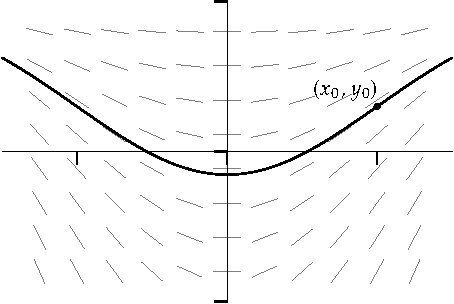
\includegraphics{figures/sampleslopes}
\caption{A \emph{slope field} giving the slope $F(x,y)$ at each point,
in this case $F(x,y)=x(1-y)$.  A solution is drawn going through the point
$(x_0,y_0)=(1,0.3)$, notice how it follows the slopes.\label{fig:sampleslopes}}
\end{myfigureht}

When $F$ involves only the $x$ variable, the solution is given by the
fundamental theorem of calculus.  On the other hand, when $F$ depends
on both $x$ and $y$ we need far more firepower.  It is not always
true that a solution exists, and if it does, that it is the unique solution.
Picard's theorem gives us certain sufficient conditions for existence
and uniqueness.

\subsection{The theorem}

We need a definition of continuity in two variables.  A point in the
plane $\R^2 = \R \times \R$ is denoted by an ordered pair $(x,y)$.
For simplicity,
we give the following sequential definition of continuity.

\begin{defn}
Let $U \subset \R^2$ be a set, $F \colon U \to \R$ a function,
and $(x,y) \in U$ a point.  The function $F$ is \emph{continuous}
\index{continuous function of two variables}
at $(x,y)$ if 
for every sequence
$\bigl\{ (x_n,y_n) \bigr\}_{n=1}^\infty$ of points in $U$ such that
$\lim_{n\to\infty} x_n = x$ and 
$\lim_{n\to\infty} y_n = y$, we have 
\begin{equation*}
\lim_{n \to \infty} F(x_n,y_n) = 
F(x,y) .
\end{equation*}
We say $F$ is continuous if it is continuous at all points in $U$.
\end{defn}

\begin{thm}[Picard's theorem on existence and uniqueness]%
\index{existence and uniqueness theorem}\index{Picard's theorem}%
\label{thm:fs:picard}
Let $I, J \subset \R$ be closed bounded intervals, 
let $I^\circ$ and $J^\circ$ be their interiors%
\footnote{By interior of $[a,b]$ we mean $(a,b)$.},
and
let $(x_0,y_0) \in I^\circ \times J^\circ$.
Suppose $F \colon I \times J \to \R$ is continuous
and Lipschitz in the second variable, that is, there exists
an $L \in \R$ such that
\begin{equation*}
\abs{F(x,y) - F(x,z)} \leq L \abs{y-z}
\qquad \text{for all } y,z \in J, x \in I .
\end{equation*}
Then there exists an $h > 0$ and a unique differentiable
function $f \colon [x_0 - h, x_0 + h] \to J \subset \R$ such that
\begin{equation} \label{picard:diffeq}
f'(x) = F\bigl(x,f(x)\bigr) \qquad \text{and} \qquad f(x_0) = y_0.
\end{equation}
\end{thm}

\begin{proof}
\pagebreak[2]
Suppose we could find a solution $f$.  Using the fundamental
theorem of calculus we integrate the equation 
$f'(x) = F\bigl(x,f(x)\bigr)$, $f(x_0) = y_0$, and write \eqref{picard:diffeq}
as the integral equation
\begin{equation} \label{picard:inteq}
f(x) = y_0 + \int_{x_0}^x F\bigl(t,f(t)\bigr)\,dt .
\end{equation}
The idea of our proof is that we try to plug in approximations to
a solution to the right-hand side of \eqref{picard:inteq} to get better approximations on the
left-hand side of  \eqref{picard:inteq}.  We hope that in the end the sequence 
converges and solves
\eqref{picard:inteq} and hence \eqref{picard:diffeq}.
The technique below is called \emph{\myindex{Picard iteration}},
and the individual functions $f_k$ are called the 
\emph{Picard iterates}\index{Picard iterate}.

Without loss of generality, suppose $x_0 = 0$ (exercise below).
Another
exercise tells us that $F$ is bounded as it is continuous.
Therefore pick some $M > 0$ so that 
$\abs{F(x,y)} \leq M$ for all $(x,y) \in I\times J$.
Pick $\alpha > 0$ such that
$[-\alpha,\alpha] \subset I$ and $[y_0-\alpha, y_0 + \alpha] \subset J$.
Define
\begin{equation*}
h \coloneqq \min \left\{ \alpha, \frac{\alpha}{M+L\alpha} \right\} .
\end{equation*}
Observe
$[-h,h] \subset I$.

Set $f_0(x) \coloneqq y_0$.
We define $f_k$ inductively.
Assuming $f_{k-1}([-h,h]) \subset [y_0-\alpha,y_0+\alpha]$,
we see 
$F\bigl(t,f_{k-1}(t)\bigr)$ is
a well-defined function of $t$ for $t \in [-h,h]$.
Further if $f_{k-1}$ is continuous
on $[-h,h]$, then
$F\bigl(t,f_{k-1}(t)\bigr)$ is
continuous as
a function of $t$ on $[-h,h]$ (left as an exercise).
Define
\begin{equation*}
f_k(x) \coloneqq y_0+ \int_{0}^x F\bigl(t,f_{k-1}(t)\bigr)\,dt ,
\end{equation*}
and $f_k$ is continuous on $[-h,h]$ by the fundamental theorem of calculus.
To see that $f_k$ maps $[-h,h]$ to $[y_0-\alpha,y_0+\alpha]$, we compute for
$x \in [-h,h]$
\begin{equation*}
\abs{f_k(x) - y_0} = 
\abs{\int_{0}^x F\bigl(t,f_{k-1}(t)\bigr)\,dt }
\leq
M\abs{x}
\leq
Mh
\leq
M
\frac{\alpha}{M+L\alpha}
\leq \alpha .
\end{equation*}
We next define $f_{k+1}$ using $f_k$ and so on.
Thus we have inductively defined a sequence $\{ f_k \}_{k=1}^\infty$ of functions.
We need to show that it converges to a function $f$ that solves
the equation~\eqref{picard:inteq} and therefore~\eqref{picard:diffeq}.

We wish to show that the sequence $\{ f_k \}_{k=1}^\infty$ converges uniformly
to some function on $[-h,h]$.  First, for $t \in [-h,h]$,
we have the following
useful bound
\begin{equation*}
\abs{F\bigl(t,f_{n}(t)\bigr) - 
F\bigl(t,f_{k}(t)\bigr)}
\leq
L \abs{f_n(t)-f_k(t)}
\leq
L \norm{f_n-f_k}_{[-h,h]} ,
\end{equation*}
where $\norm{f_n-f_k}_{[-h,h]}$ is the uniform norm, that
is the supremum of $\abs{f_n(t)-f_k(t)}$ for $t \in [-h,h]$.
Now note that $\abs{x} \leq h \leq \frac{\alpha}{M+L\alpha}$.
Therefore
\begin{equation*}
\begin{split}
\abs{f_n(x) - f_k(x)}
& =
\abs{\int_{0}^x F\bigl(t,f_{n-1}(t)\bigr)\,dt 
-
\int_{0}^x F\bigl(t,f_{k-1}(t)\bigr)\,dt}
\\
& =
\abs{\int_{0}^x F\bigl(t,f_{n-1}(t)\bigr)-
F\bigl(t,f_{k-1}(t)\bigr)\,dt}
\\
& \leq
L\norm{f_{n-1}-f_{k-1}}_{[-h,h]}
\abs{x}
\\
& \leq
\frac{L\alpha}{M+L\alpha}
\norm{f_{n-1}-f_{k-1}}_{[-h,h]} .
\end{split}
\end{equation*}
Let $C \coloneqq \frac{L\alpha}{M+L\alpha}$ and note that $C < 1$.
Taking supremum on the left-hand side we get
\begin{equation*}
\norm{f_n-f_k}_{[-h,h]} \leq C \norm{f_{n-1}-f_{k-1}}_{[-h,h]} .
\end{equation*}
Without loss of generality,
suppose $n \geq k$.  Then by \hyperref[induction:thm]{induction} we can show 
\begin{equation*}
\norm{f_n-f_k}_{[-h,h]} \leq C^{k} \norm{f_{n-k}-f_{0}}_{[-h,h]} .
\end{equation*}
For $x \in [-h,h]$, we have
\begin{equation*}
\abs{f_{n-k}(x)-f_{0}(x)}
=
\abs{f_{n-k}(x)-y_0}
\leq \alpha .
\end{equation*}
Therefore,
\begin{equation*}
\norm{f_n-f_k}_{[-h,h]} \leq C^{k} \norm{f_{n-k}-f_{0}}_{[-h,h]} \leq C^{k} \alpha .
\end{equation*}
As $C < 1$, $\{f_n\}_{n=1}^\infty$ is uniformly Cauchy and by
\propref{prop:uniformcauchy} we obtain that $\{ f_n \}_{n=1}^\infty$
converges uniformly on $[-h,h]$ to some function $f \colon [-h,h] \to \R$.
The function $f$ is the uniform limit of continuous functions and therefore
continuous.  Furthermore, since $f_n\bigl([-h,h]\bigr) \subset
[y_0-\alpha,y_0+\alpha]$ for all $n$,
then $f\bigl([-h,h]\bigr) \subset [y_0-\alpha,y_0+\alpha]$
(why?).


We now need to show that $f$ solves \eqref{picard:inteq}.
First, as before we notice
\begin{equation*}
\abs{F\bigl(t,f_{n}(t)\bigr) - 
F\bigl(t,f(t)\bigr)}
\leq
L \abs{f_n(t)-f(t)}
\leq
L \norm{f_n-f}_{[-h,h]} .
\end{equation*}
As $\norm{f_n-f}_{[-h,h]}$ converges to 0, then
$F\bigl(t,f_n(t)\bigr)$ converges uniformly to $F\bigl(t,f(t)\bigr)$
for $t \in [-h,h]$.  Hence, for $x \in [-h,h]$
the convergence is uniform %(why?)
for $t \in [0,x]$ (or $[x,0]$ if $x < 0$).  Therefore,
\begin{align*}
y_0
+
\int_0^{x}
F(t,f(t)\bigr)\,dt
& =
y_0
+
\int_0^{x}
F\bigl(t,\lim_{n\to\infty} f_n(t)\bigr)\,dt
& &
\\
& =
y_0
+
\int_0^{x}
\lim_{n\to\infty} F\bigl(t,f_n(t)\bigr)\,dt
& & \text{(by continuity of } F\text{)}
\\
& =
\lim_{n\to\infty} 
\left(
y_0
+
\int_0^{x}
F\bigl(t,f_n(t)\bigr)\,dt
\right)
& & \text{(by uniform convergence)}
\\
& =
\lim_{n\to\infty} 
f_{n+1}(x)
=
f(x) .
& &
\end{align*}
We apply the fundamental theorem of calculus (\thmref{thm:FTCv2}) to show that
$f$ is differentiable and its derivative is $F\bigl(x,f(x)\bigr)$.  It is obvious
that $f(0) = y_0$.

Finally, what is left to do is to show uniqueness.  Suppose $g \colon [-h,h]
\to J \subset \R$ is another solution.
As before we use the fact that
$\abs{F\bigl(t,f(t)\bigr) - F\bigl(t,g(t)\bigr)} \leq L \norm{f-g}_{[-h,h]}$.
Then
\begin{equation*}
\begin{split}
\abs{f(x)-g(x)}
& =
\abs{
y_0
+
\int_0^{x}
F\bigl(t,f(t)\bigr)\,dt
-
\left(
y_0
+
\int_0^{x}
F\bigl(t,g(t)\bigr)\,dt
\right)
}
\\
& =
\abs{
\int_0^{x}
F\bigl(t,f(t)\bigr)
-
F\bigl(t,g(t)\bigr)\,dt
}
\\
& \leq
L\norm{f-g}_{[-h,h]}\abs{x}
\leq
Lh\norm{f-g}_{[-h,h]}
\leq
\frac{L\alpha}{M+L\alpha}\norm{f-g}_{[-h,h]} .
\end{split}
\end{equation*}
As 
before, $C = \frac{L\alpha}{M+L\alpha} < 1$.  By taking supremum over $x \in
[-h,h]$ on the
left-hand side we obtain
\begin{equation*}
\norm{f-g}_{[-h,h]} \leq C \norm{f-g}_{[-h,h]} .
\end{equation*}
This is only possible if $\norm{f-g}_{[-h,h]} = 0$.  Therefore, $f=g$, and the
solution is unique.
\end{proof}

\subsection{Examples}

Let us look at some examples.  The proof of the theorem 
gives us an explicit way to find an $h$ that works.  It does not, however, give
us the best $h$.  It is often possible to find a much larger $h$ for
which the conclusion of the theorem holds.

The proof also gives us the Picard iterates as approximations to the
solution.  So the proof actually tells us how to obtain
the solution, not just that the solution exists.

\begin{example} \label{example:picardexponential}
Consider
\begin{equation*}
f'(x) = f(x), \qquad f(0) = 1 .
\end{equation*}
That is, we suppose $F(x,y) = y$, and we are looking for a function 
$f$ such that $f'(x) = f(x)$.
Let us forget for the moment that we solved this equation in 
\sectionref{sec:logandexp}.  See also \figureref{fig:exp} for a plot of
both the equation, showing
the slope $F(x,y)=y$ at each point, and the solution,
the exponential, that satisfies $f(0)=1$.

We pick any $I$ that contains 0
in the interior.
We pick an arbitrary $J$ that contains 1 in its interior.  We can
use $L = 1$.
The theorem guarantees an $h > 0$ such that
there exists a unique solution $f \colon [-h,h] \to \R$.  This solution
is usually denoted by
\begin{equation*}
e^x \coloneqq f(x) .
\end{equation*}
We leave it to the reader to verify that by picking $I$ and $J$
large enough the proof of the theorem guarantees that
we are able to pick $\alpha$ such that we get any
$h$ we want as long as $h < \nicefrac{1}{2}$.  We omit the calculation.

Of course, we know %(though we have not proved)
this function exists
as a function for all $x$, so an arbitrary $h$ ought to work.
By same reasoning as above,
no matter what $x_0$ and $y_0$ are,
the proof guarantees an arbitrary $h$ as long as $h < \nicefrac{1}{2}$.
Fix such an $h$.
We get a unique function defined on $[x_0-h,x_0+h]$.  After defining the
function on $[-h,h]$ we find a solution on the interval $[0,2h]$
and notice that the two functions must coincide on $[0,h]$ by uniqueness.
We thus iteratively construct the exponential for all $x \in \R$.
Therefore Picard's theorem could be used to prove the existence and uniqueness
of the exponential.

Let us compute the Picard iterates.
We start with the constant function $f_0(x) \coloneqq 1$.  Then
\begin{align*}
f_1(x) & = 1 + \int_0^x f_0(s)\,ds =
1+x, \\
f_2(x) & = 1 + \int_0^x f_1(s)\,ds =
1 + \int_0^x (1+s)\,ds = 1 + x + \frac{x^2}{2}, \\
f_3(x) & = 1 + \int_0^x f_2(s)\,ds =
1 + \int_0^x \left(1+ s + \frac{s^2}{2} \right)\,ds =
1 + x + \frac{x^2}{2} + \frac{x^3}{6} .
\end{align*}
We recognize the beginning of the Taylor series for the exponential.
See \figureref{fig:exppicard}.
\begin{myfigureht}
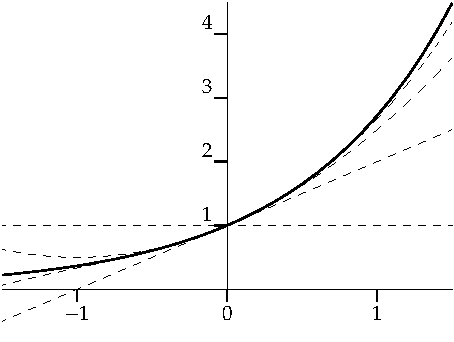
\includegraphics{figures/exppicardfig}
\caption{The exponential (solid line) together with $f_0$, $f_1$, $f_2$,
$f_3$ (dashed).\label{fig:exppicard}}
\end{myfigureht}
\end{example}

\begin{example}
Consider the equation
\begin{equation*}
f'(x) = {\bigl(f(x)\bigr)}^2 \qquad \text{and} \qquad f(0)=1.
\end{equation*}
From elementary differential equations we know 
\begin{equation*}
f(x) = \frac{1}{1-x}
\end{equation*}
is the solution.
The solution is only defined on $(-\infty,1)$.  That is,
we are able to use $h < 1$, but never a larger $h$.
The function that takes $y$ to $y^2$ is
not Lipschitz as a function on all of $\R$.
As we approach $x=1$ from the left, the solution becomes larger
and larger.  The derivative of the solution grows as $y^2$, and so
the $L$ required has to be larger and larger as $y_0$ grows.
If we apply the
theorem with $x_0$ close to 1 and $y_0 = \frac{1}{1-x_0}$ we find
that the $h$ that the proof guarantees is smaller and smaller as $x_0$
approaches 1.

The $h$ from the proof is not the best $h$.
By picking $\alpha$ correctly, the proof of the theorem guarantees
$h=1-\nicefrac{\sqrt{3}}{2} \approx 0.134$ (we omit the
calculation) for $x_0=0$ and $y_0=1$, even though
we saw above that any $h < 1$ should work.
\end{example}

\begin{example}
Consider the equation
\begin{equation*}
f'(x) = 2 \sqrt{\abs{f(x)}}, \qquad f(0) = 0 .
\end{equation*}
The function $F(x,y) = 2 \sqrt{\abs{y}}$ is continuous,
but not Lipschitz in $y$ (why?). 
The equation does not satisfy the hypotheses of the theorem.
The function
\begin{equation*}
f(x) =
\begin{cases}
x^2 & \text{if } x \geq 0,\\
-x^2 & \text{if } x < 0,
\end{cases}
\end{equation*}
is a solution, but $f(x) = 0$ is also a solution.
A solution exists, but is not unique.
\end{example}

\begin{example}
Consider $y' = \varphi(x)$ where $\varphi(x) \coloneqq 0$ if $x \in \Q$ and
$\varphi(x)\coloneqq 1$ if $x
\not\in \Q$.  In other words, the $F(x,y) = \varphi(x)$ is discontinuous.
The equation has no solution regardless of the initial
conditions.
A solution would have
derivative $\varphi$, but $\varphi$ does not have the intermediate value property
at any point (why?).  No solution exists by
\hyperref[thm:darboux]{Darboux's theorem}.
\end{example}

The examples show that without the Lipschitz condition, a solution might
exist but not be a unique, and without continuity of $F$, we may not
have a solution at all.
It is in fact a theorem, the Peano existence theorem, that if $F$ is
continuous a solution exists (but may not be unique).

\begin{remark}
It is possible to weaken what we mean by \myquote{solution to $y' = F(x,y)$}
by focusing on the integral equation
$f(x) = y_0 + \int_{x_0}^x F\bigl(t,f(t)\bigr) \, dt$.  For example,
let $H$ be the
Heaviside function%
\footnote{Named
for the English engineer, mathematician, and physicist
\href{https://en.wikipedia.org/wiki/Oliver_Heaviside}{Oliver Heaviside}
(1850--1825).},
that is $H(t) \coloneqq 0$ for $t < 0$ and $H(t) \coloneqq 1$ for $t \geq 0$.
Then
$y' = H(t)$, $y(0) = 0$,
is a common equation.
The \myquote{solution}
is the ramp function $f(x) \coloneqq 0$ if $x < 0$ and $f(x) \coloneqq x$ if $x \geq 0$,
since this function satisfies
$f(x) = \int_0^x H(t)\, dt$.  Notice, however, that $f'(0)$ does not exist,
so $f$ is only a so-called \emph{\myindex{weak solution}} to the
differential equation.
\end{remark}


\subsection{Exercises}

\begin{exercise}
Let $I, J \subset \R$ be intervals.
Let $F \colon I \times J \to \R$ be a continuous function
of two variables
and suppose $f \colon I \to J$ be a continuous function.
Show that $F\bigl(x,f(x)\bigr)$ is a continuous function on $I$.
\end{exercise}

\begin{exercise}
Let $I, J \subset \R$ be closed bounded intervals.
Show that if $F \colon I \times J \to \R$ is continuous,
then $F$ is bounded.
\end{exercise}

\begin{exercise}
We proved Picard's theorem under the assumption that $x_0 = 0$.
Prove the full statement of Picard's theorem for an arbitrary $x_0$.
\end{exercise}

\begin{exercise}
Let $f'(x)=x f(x)$ be our equation.  Start with the initial condition
$f(0)=2$ and find the Picard iterates $f_0,f_1,f_2,f_3,f_4$.
\end{exercise}

\begin{exercise}
Suppose $F \colon I \times J \to \R$
is a function that is continuous in the first variable,
that is, for every fixed $y$ the function that takes $x$ to $F(x,y)$ is
continuous.  Further, suppose $F$ is Lipschitz in the second variable,
that is, there exists a number $L$ such that
\begin{equation*}
\abs{F(x,y) - F(x,z)} \leq L \abs{y-z}
\qquad \text{for all } y,z \in J, x \in I .
\end{equation*}
Show that $F$ is continuous as a function of two variables.  Therefore, the
hypotheses in the theorem could be made even weaker.
\end{exercise}

\begin{exercise}
\pagebreak[2]
A common type of equation one encounters are
\emph{\myindex{linear first order differential equations}}, that is
equations of the form
\begin{equation*}
y' + p(x) y = q(x) , \qquad y(x_0) = y_0 .
\end{equation*}
Prove Picard's theorem for linear equations.  Suppose $I$ is an
interval, $x_0 \in I$, and $p \colon I \to \R$ and $q \colon I \to \R$ are
continuous.
Show that there exists a unique differentiable $f \colon I \to \R$,
such that $y = f(x)$
satisfies the equation and the initial condition.
Hint: Assume existence of the exponential function and use the integrating
factor formula for existence of $f$ (prove that it works and then that it is unique):
\begin{equation*}
f(x) \coloneqq e^{-\int_{x_0}^x p(s)\, ds} \left( \int_{x_0}^x e^{\int_{x_0}^t p(s)\, ds}
q(t) \,dt + y_0 \right).
\end{equation*}
\end{exercise}

\begin{exercise}
Consider the equation $f'(x) = f(x)$,
from \exampleref{example:picardexponential}.  Show that given any $x_0$,
any $y_0$, and any positive $h < \nicefrac{1}{2}$, we can pick $\alpha >
0$ large enough that the proof of Picard's theorem guarantees a solution
for the initial condition $f(x_0) = y_0$ in the interval
$[x_0-h,x_0+h]$.
\end{exercise}

\begin{exercise}
\pagebreak[3]
Consider the equation $y' = y^{1/3}x$.
\begin{enumerate}[a)]
\item
Show that for the initial condition $y(1)=1$, Picard's theorem applies.
Find an $\alpha > 0$, $M$, $L$, and $h$ that would work in the proof.
\item
Show that for the initial condition $y(1) = 0$, Picard's theorem
does not apply.
\item
Find a solution for $y(1) = 0$ anyway.
\end{enumerate}
\end{exercise}

\begin{exercise}
Consider the equation $x y' = 2y$.
\begin{enumerate}[a)]
\item
Show that $y = Cx^2$ is a solution for every constant $C$.
\item
Show that for every $x_0 \not= 0$ and every $y_0$, Picard's
theorem applies for the initial condition $y(x_0) = y_0$.
\item
Show that $y(0) = y_0$ is solvable if and only if $y_0 = 0$.
\end{enumerate}
\end{exercise}
